\documentclass[../thesis.tex]{subfiles}

\begin{document}

Steady progress in any modern scientific endeavor requires a strong, dynamic relationship between experimental data to paint an accurate picture of some natural phenomena and theoretical models to interpret those phenomena with respect to the growing network of other scientific models. Conversely, the predictive capability of theoretical models can highlight blurry or unfinished areas of that picture which can be clarified or completed by new or improved experimental techniques. In the pursuit to understand and describe the atomic nucleus and the corresponding implications from quarks to neutron stars, this push-and-pull coordination between theory and experiment makes progress in modern nuclear physics robust and persistent.

An integral component of modern nuclear physics is describing the structure and emergent properties of self-bound systems of protons and neutrons. The systems in questions can be stable nuclei, rare isotopes far from stability, and even infinite nuclear matter which can be used to model neutron stars. Relevant properties to nuclear structure include ground-state energies--for determining nuclear masses, excited-state energies--for identification in gamma or neutron spectroscopy, and transition or decay amplitudes--for calculating the respective rates for those processes. This wide array of emergent properties inserts both nuclear structure theory and experiment into a prominent role within every other subfield of modern nuclear physics, from lattice quantum chromodynamics (QCD) to nuclear astrophysics, and beyond, to questions about fundamental symmetries and dark matter.  However, two inextricable characteristics of a comprehensive model of nuclear structure--the increasingly large size of many-body nuclear systems and the complexity and strength of the nucleon-nucleon interactions--have been imposing hurdles for theorists to overcome.


\section{A Brief History of Nuclear Structure Theory}

The project to solve the correlation problem in many-fermion systems began with the work of Brueckner, Bethe, and Goldstone \cite{BRUECKNER19551344,BETHE19561353,GOLDSTONE1957267} with the reformulation of the nuclear interaction by accounting for two-body correlations from the nuclear medium.  This work continued with the work of Coester \cite{COESTER1958421,COESTER1960477} and Kummel \cite{KUMMEL19781}, amongst many other, with a further resummation of nuclear correlations in the form of an exponential ansatz into what would become coupled-cluster (CC) theory.  However, there were two major obstacles that hindered the progress in this area for decades.  First, while these methods were systematically improvable by including progressively higher-level correlations, the highly nonperturbative nature of the nuclear force required computationally infeasible summations.  Second, there wasn't a reliable and consistent theory to model nucleon-nucleon interactions.

However, with the well-known and highly-perturbative Coulomb force, which underlies the many-electron systems in atoms and molecules, the field of quantum chemistry made consistent advances in ab-initio quantum chemistry possible since the 1950s.  Along with the quasi-exact method of configuration interaction (CI) theory \cite{SLATER19291293,CONDON19301121,BACHER1933264,UFFORD1933732} which have been utilized since the formulation of quantum mechanics, chemists successfully employed approximate methods like many-body perturbation theory (MBPT) \cite{HUBBARD1957539,HUGENHOLTZ1957481,SCHAEFER1984,SHAVITT2009} and coupled-cluster theory \cite{CIZEK19664256,CIZEK1971359,CIZEK1980251,PIECUCH2002527,SHAVITT2009}.

\begin{figure}[h]
  \centering
  \begin{subfigure}{0.7\textwidth}
    \centering
    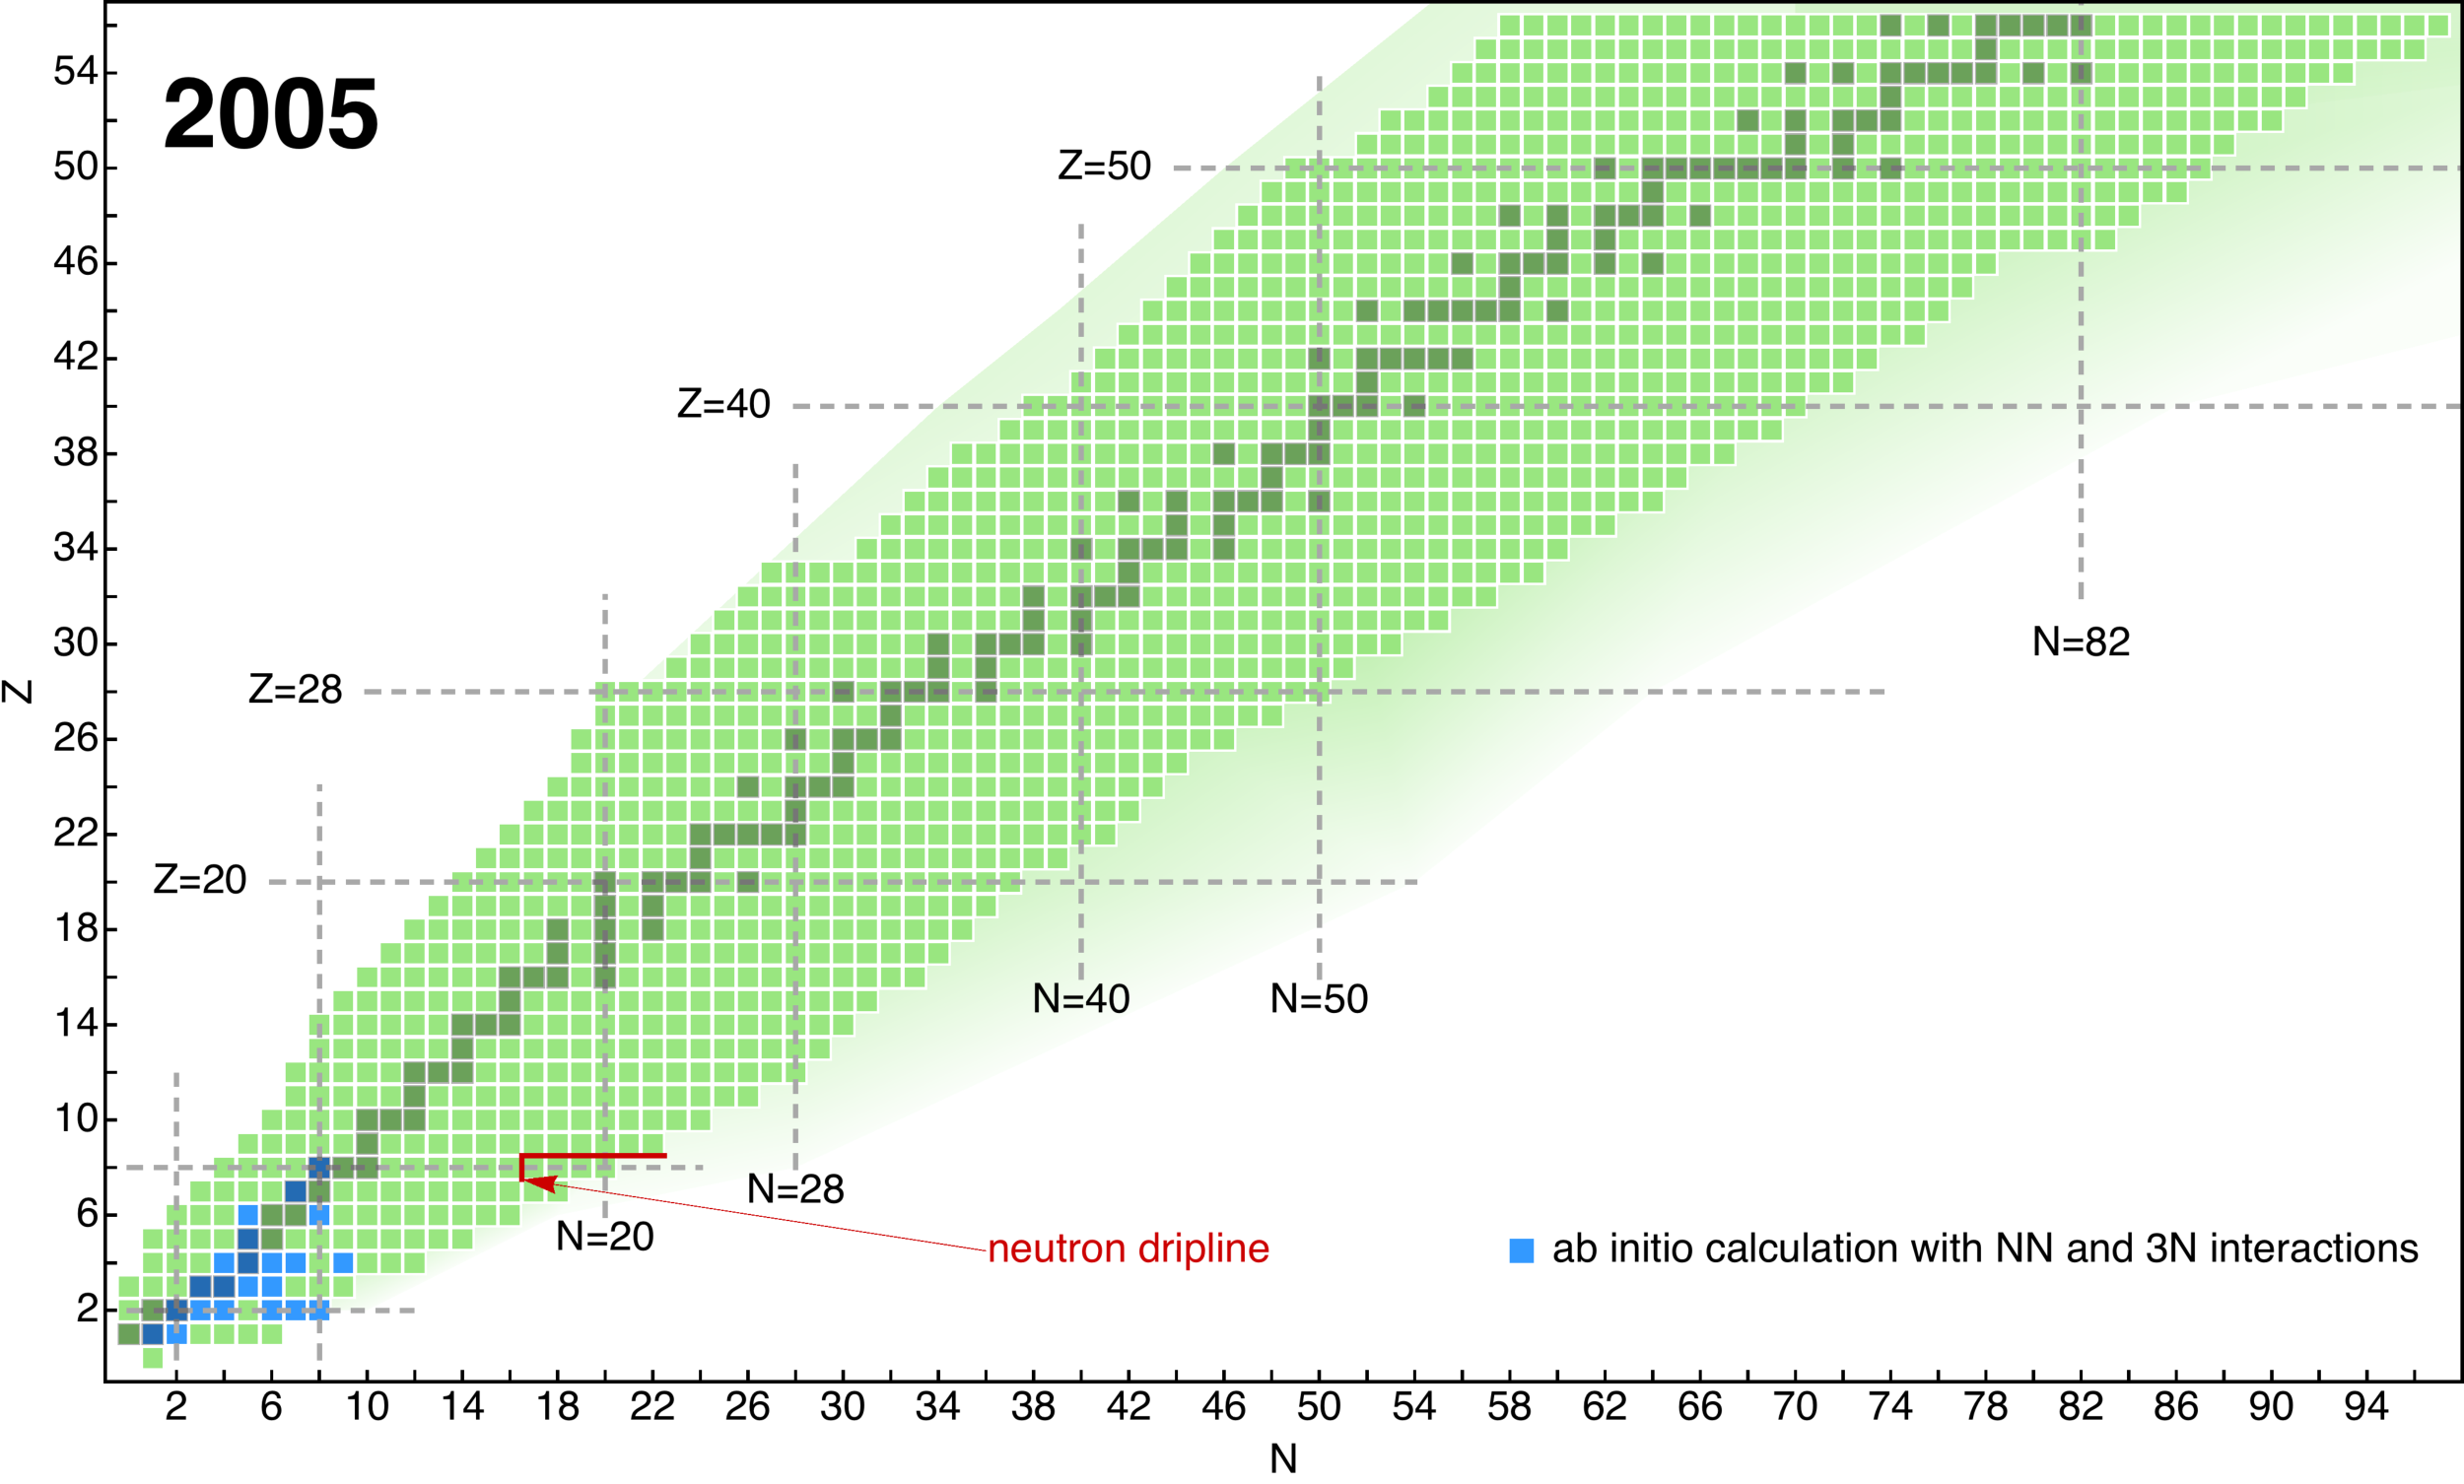
\includegraphics[width=\textwidth]{introduction/ab-initio_nuclear_chart_2005.pdf}
  \end{subfigure}
  
  \begin{subfigure}{0.7\textwidth}
    \centering
    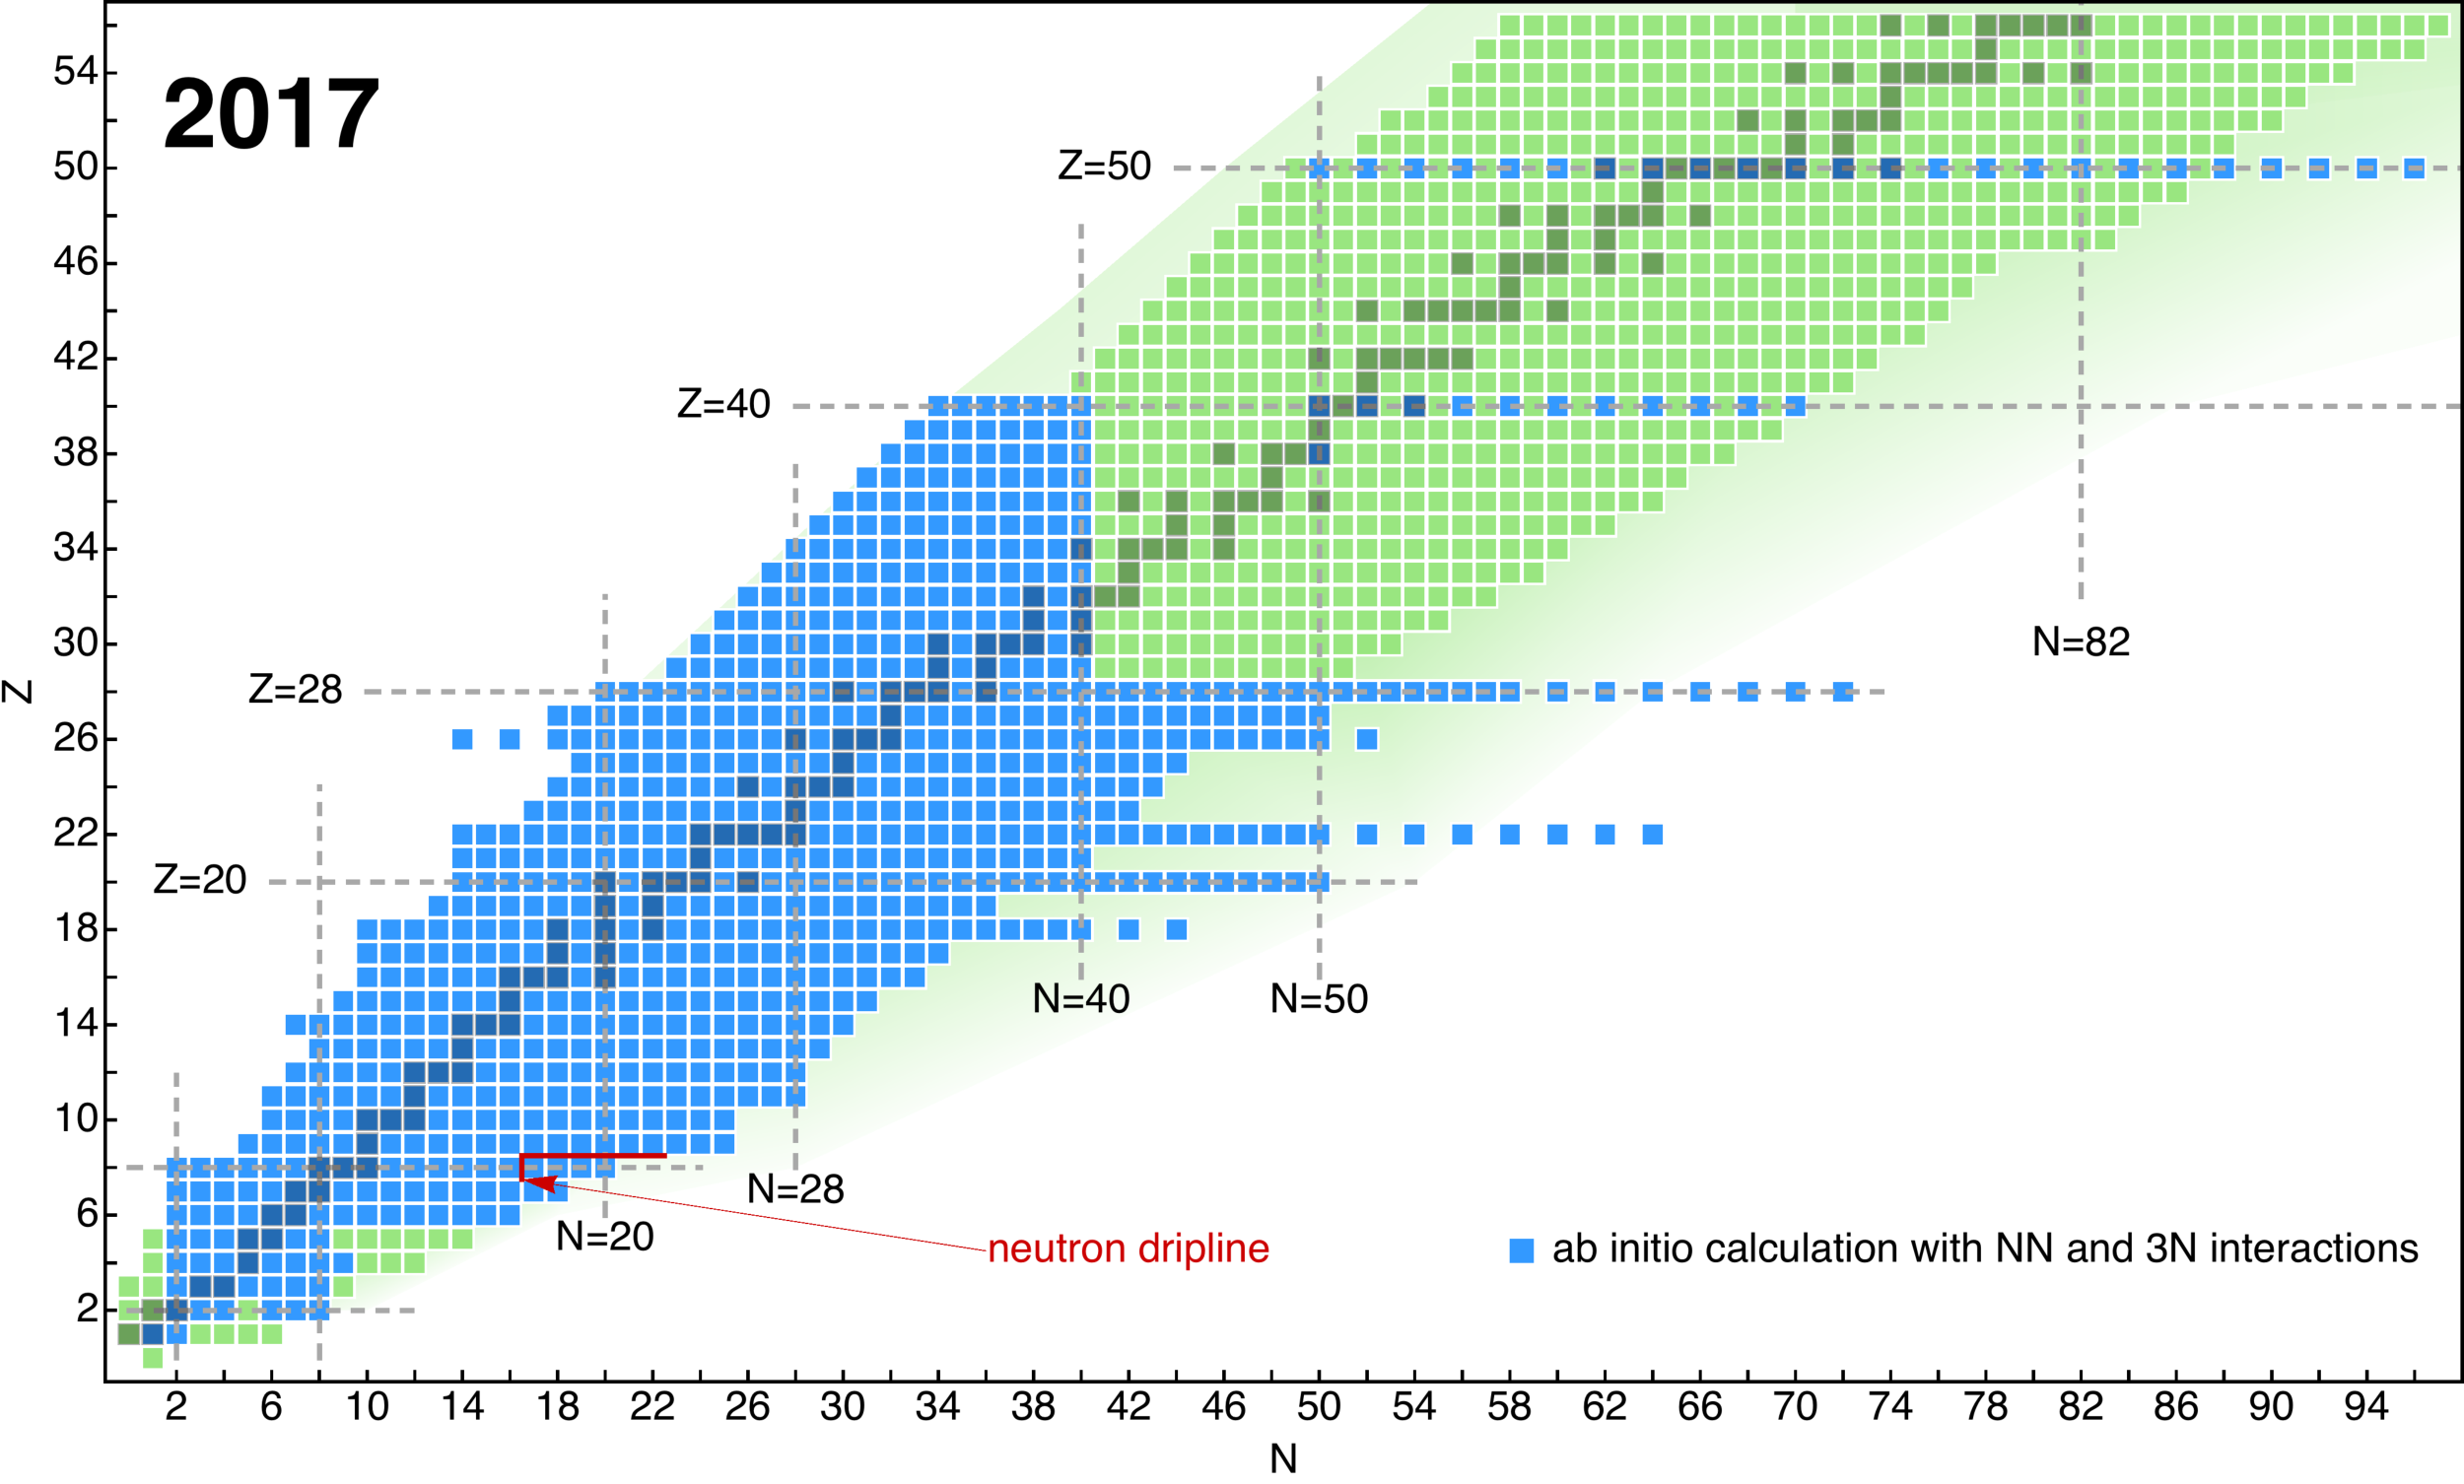
\includegraphics[width=\textwidth]{introduction/ab-initio_nuclear_chart_2017.pdf}
  \end{subfigure}
  \caption{Nuclear chart of nuclei with ground-state energies which have been calculated with ab-initio methods and NN+3N interactions.  Figure taken from \cite{HERGERTPRIVATE}.}
  \label{fig:AbInitioChart}
\end{figure}

Fortunately, within the past decade, two breakthroughs have allowed \emph{ab initio} nuclear structure to resurface and thrive the way that quantum chemistry had done in the previous decades.  First was the invention of chiral effective field theory (EFT) \cite{EPELBAUM20091773,MACHLEIDT20111} which gave theorists the ability to construct nucleon-nucleon interactions consistent with the underlying QCD of the strong nuclear force.  Second was the application of renormalization group (RG) methods to the nuclear force \cite{BOGNER201094,ROTH2011072501}.  This procedure can ``soften'' the NN interaction, to decouple the high- and low-momentum components of the nuclear force and generate less-correlated systems that can be calculated at a reasonable computational cost.  These major changes to nuclear structure theory made it possible to merge the field with the progress of quantum chemistry and open a new area for additional developments in \emph{ab initio} descriptions of many-fermion systems, see Fig.\ \ref{fig:AbInitioChart}.

Along with exponential improvements to high-performance computing, these novel techniques have allowed modern many-body methods to extend their reach and deepen their applicability across the nuclear chart, see Fig.\ \ref{fig:AbInitioProgress}.  The no-core shell model (NCSM), an exact method for a given model space, has been useful in calculating the radii, transition strengths, and effective interactions of light nuclei and has been extended to nuclei in the $sd$ shell \cite{NAVRATIL2000054311,NAVRATIL2009083101,BARRETT2013131}.  A quasi-exact technique which follows a completely different methodology than NCSM, quantum Monte Carlo (QMC), has also progressed and is now capable of calculating properties of light nuclei with modern chiral forces \cite{PUDLINER19971720,PIEPER200153,CARLSON20151067}.  In addition to these exponentially scaling techniques' successes with lighter nuclei, polynomially scaling techniques--such as the in-medium similarity renormalization group (IMSRG) \cite{TSUKIYAMA2011222502,TSUKIYAMA2012061304,HERGERT2013242501,BOGNER2014142501,HERGERT2014041302,HERGERT2017023002,STROBERG2016051301,STROBERG2017032502}, self-consistent Green's functions (SCGF) \cite{SOMA2013011303,SOMA2014024323,SOMA2014061301}, and coupled cluster theory \cite{WLOCH2005212501,WLOCH2005S1291,JANSEN2014142502,JANSEN2016011301,HAGEN2015186,KOWALSKI2004132501,GOUR2006024310,BINDER2013054319}--have been able to reach open-shell nuclei through the $pf$ shell and even up to the chain of even tin isotopes with equations-of-motion and multi-reference techniques \cite{MORRIS2017}.

\begin{figure}[h]
  \centering
  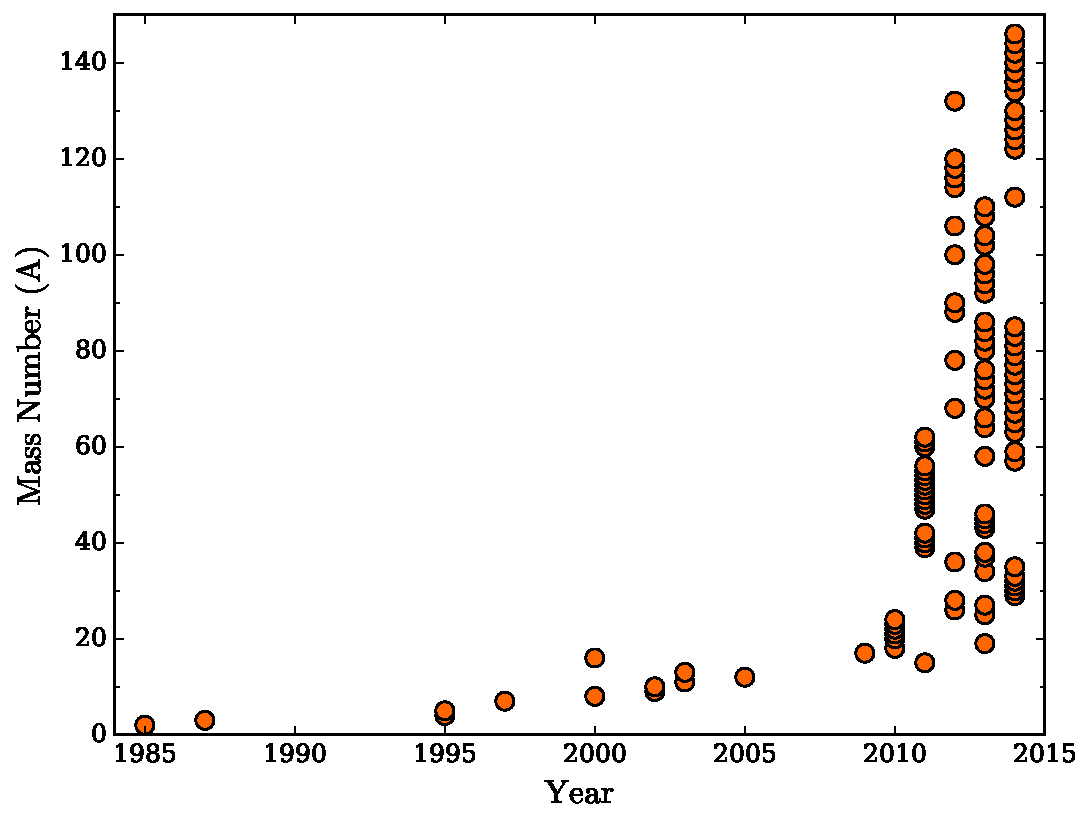
\includegraphics[width=0.75\textwidth]{introduction/ab-initio_progress.pdf}
  \caption{Progress of ab-initio nuclear structure from calculations of ground-state energies with NN+3N interactions.  Early progress was approximately linear as the problem size scaled with Moore's law while more recent progress has taken advantage of new algorithms which have outpaced Moore's law.  Data taken from \cite{HERGERTPRIVATE}.}
  \label{fig:AbInitioProgress}
\end{figure}


\section{Electroweak Theory and Nuclear Structure}

Nuclear structure is implicated in performing and analyzing experiments to probe fundamental symmetries and physics beyond the Standard Model. One example is determining the $\mathrm{V_{ud}}$ component of the Cabibbo-Kobayashi-Maskawa (CKM) matrix, which relates quark eigenstates of the weak interaction to their mass eigenstates \cite{CABBIBO1963531,KOBAYASHI1973652}. This component can be determined from by measuring the half-lives of superallowedbeta decays \cite{TOWNER2003197} and applying a nucleus-dependent structure correction \cite{TOWNER2008025501,TOWNER199413,TOWNER1992478,BARKER1992501,JAUS1990166}. The value of $\left|\mathrm{V_{ud}}\right|$ is used to test the unitarity of the CKM matrix and the conserved-vector current hypothesis, which relates the $f$t-values of superallowed Fermi $\beta$ decays of different nuclei, both predicted by the standard model \cite{HARDY2005055501}.

Another example of physics beyond the standard model is the neutrinoless double-beta decay ($0\nu\beta\beta$) \cite{SUHONEN1998123,AVIGNONE2008481}. The extremely-rare, two-neutrino double-beta decay ($2\nu\beta\beta$) has been observed in many experiments \cite{ELLIOTT19872020,MILEY19903092}, which has motivated the search for its neutrinoless counterpart, in which two Majorana neutrinos, being their own antiparticles, annihilate one another, which is not possible in the standard electro-weak theory. The long half-lives of these theoretical decays depend on a phase-space factor, which is highly dependent on the decay $Q$-value, and a nuclear matrix element. The $Q$-value can be determined from high-precision mass measurements of the relevant nuclei \cite{LINCOLN2013012501,GULYUZ2015055501,REDSHAW2012041306,BUSTABAD2013022501}, while the nuclear matrix element, which contributes the largest source of uncertainty, must be calculated with a reliable many-body theory. 

The weak interaction and nuclear structure can also be exploited for supernova neutrino detection and spectroscopy. While these original detectors were based on electron-neutrino scattering \cite{HIRATA19871490,BIONTA19871494}, more recent experiments utilize correlated nucleon effects of large nuclei to enhance the scattering cross section and therefore the ability to resolve energies and distinguish neutrino flavors \cite{HARGROVE1996183,CLINE1994720,EWAN1992373,LANGANKE19962629}. Supernova models predict distinct distributions for different neutrino flavors based on the temperatures at which they are emitted \cite{KOLBE20032569,BENHAR2005053005}. With nuclear structure calculations that include sufficient nuclear correlations, these high-resolution detectors can be used to verify specific models.


\section{Ab-Initio Descriptions of Beta Decay}

Since Enrico Fermi's originally rejected paper describing beta decay in 1934 \cite{FERMI1934,WILSON1968}, theorists have worked to refine this description within the ever-growing library of knowledge concerning the nature of the weak force, the characteristics of the neutrino, and the structure of nuclei.  With the success of \emph{ab initio} calculations for nuclear properties such as masses, radii, and electromagnetic phenomena, these techniques also seem promising ways to calculate relevant quantities involved in nuclear beta decay.  Because the kinematics of the decay and the underlying weak process are well understood, the remaining task for nuclear theory to tackle is calculating the transition amplitudes between the initial and final nuclei.

Modern calculations of these beta-decay matrix elements were originally performed using phenomenological interactions in the shell model framework \cite{WILDENTHAL1983,BROWN1983,WARBURTON1992,ORMAND1995}.  Also, predecessors to current ab-initio techniques like the random-phase approximation (RPA) \cite{TOWNER1979} included core-correlation effects in these early descriptions.  These methods were able to successfully reproduce experimental lifetime data and address technical issues such as the quenching of the axial-vector coupling constant.  More recently, the success of the shell model has inspired an extension to the new method, known as the ab-initio shell model \cite{BARRETT2013131}, where an effective interaction is constructed within a certain valence space using a many-body method such as CC \cite{JANSEN2014} or IMSRG \cite{BOGNER2014}.  However, these techniques are computationally expensive and cannot currently reach heavy nuclei of interest.  The most common method used in their place is known as the quasiparticle random-phase approximation (QRPA) \cite{SUHONEN2013153,ENGEL2015}.  While these calculations can be performed for heavy nuclei in large spaces, they also rely on phenomenological effective interactions.  Therefore, there is a demand for computationally-economical, \emph{ab initio} techniques that can capture the relevant many-body correlations needed to accurately describe the nuclear structure aspects of electro-weak processes.



\section{Thesis Structure}

The main goal of this work is to explore the \emph{ab initio} description of nuclear beta decay within the coupled-cluster theory framework of the \textit{equation-of-motion coupled cluster with singles and doulbes} (EOM-CCSD) method using renormalized chiral NN and 3N interactions.  The organization of the thesis builds from a general description of the many-body problem of quantum mechanics in chapter \ref{chapter:manybody}. Then, in chapter \ref{chapter:cc}, this many-body framework is applied within the coupled-cluster theory and applied to various systems including, atomic nuclei. In chapter \ref{chapter:eom}, coupled-cluster theory is extended to the equations-of-motion method to describe open-shell systems.  Then, in chapter \ref{chapter:betadecay}, different types of beta decay are described in detail then outlines the procedure to express beta-decay observables as effective coupled-cluster operators and how to calculate those observables in the equations-of-motion framework.  Lastly, conclusions and future perspectives are given in chapter \ref{chapter:conclusions} while technical details concerning the formalism and implementation are given in the appendices \ref{chapter:ccsd_appendix} -- \ref{chapter:angular_momentum}.

\end{document}
